\chapter{Evaluation}\label{C:us}

Following the completed scraper implementation and data analysis, an evaluation of the project was carried out on both the scrapers and policies. The evaluation was designed primarily to verify whether or not the scraper and policies created were succesful in fulfilling the requirements of the project. The following aspects of the IHPScrape framework were evaluated: accuracy, performance, resistance to user interface change, and  resistance to detection. 

\section{Scraper Accuracy}

Requirement NF3 stated that data gathered needs to be accurate in order to generate meaningful results, and that any potential innacuracies in data collected should be well understood. Quantitatively evaluating the accuracy of figures gathered by IHPScrape was difficult without a dataset to compare results against. Given that one of the primary reasons for implementing a scraper was due to this lack of a valid dataset, such an evaluation was not possible within the time constraints of the project.  As such I performed a qualitative evaluation of aspects of scraper accuracy. 

To measure relative scraper accuracy, manual inspection of 15 random Twitter profiles that were fetched in the final build was conducted. Figure 7.1 displays the data checked for accuracy on the user's Twitter profile pages, and scraped xml file. Details checked for correctness were as follows:

\begin{itemize}
 \item The number of users following the test subject (Number of Followers Correct)
 \item The number of users the subject follows (Number of Following Correct)
 \item The number of posts by the users (Number of Tweets Correct)
 \item Whether retweet counts recorded were accurate (Retweet Counts Accurate)
 \item Whether the set of profile names recorded as retweeting a post was correct and complete (Retweeter Names Correct)
 \item Whether the entire set of tweets posted by the subject were collected (Tweet List Complete)
\end{itemize}

\begin{sidewaysfigure}[p]
\begin{center}
 \begin{tabular}{| p{3cm} | p{3cm}| p{3cm} | p{3cm} | p{3cm} | p{3cm} | p{2cm} |}
 \hline
 \textbf{Profile Name} & \textbf{Number of Followers Correct} & \textbf{Number Following Correct} & \textbf{Number of Tweets Correct} & \textbf{Retweet counts accuracte} & \textbf{Retweeter Names Correct} & \textbf{Tweet List Complete}\\ \hline
\_Eduardofficial & Yes & Yes & Yes & Yes & Incomplete & Yes\\ \hline
 MichaelaCNN & Yes & Yes & Yes & Yes & Incomplete & Yes \\ \hline
 Natalyacoyle & Yes & Yes & Yes & Yes & Incomplete & Yes \\ \hline
 OpheliaDagger & Yes & Yes & Yes & Yes & Incomplete & Yes \\ \hline
 NitaLowey & Yes & Yes & Yes & Yes & Yes & Yes  \\ \hline
 mims & Yes & Yes & Yes & Yes & Incomplete & No \\ \hline
 sherlynroy & Yes & Yes & Yes & Yes & Yes & Yes \\ \hline
 Natpolitic & Yes & Yes & Yes & Yes & Yes & Yes \\ \hline
 portereduardo & Yes & Yes & Yes & Yes & Yes & Yes \\ \hline
 NatbyNature & Yes & Yes & Yes & Yes & Incomplete & No \\ \hline
 NewzMuse & Yes & Yes & Yes & Yes & Yes & Yes \\ \hline
 NitaLakeLodge & Yes & Yes & Yes & Yes & Yes & Yes \\ \hline
 MirellaVieiraa & Yes & Yes & Yes & Yes & Yes & No \\ \hline
 JanuarySeraph & Yes & Yes & Yes & Yes & Incomplete & No \\ \hline
 MissKacieMarie & Yes & Yes & Yes & Yes & Incomplete & No \\ \hline
 \end{tabular}
\end{center}
\caption{Accuracy Metric Results}
\end{sidewaysfigure}

The results of this sample test were encouraging. Static and unchanging values such as Number of followers, number following, and number of tweets were always correct. Dynamic lists such as the retweet names were sometimes incomplete. This was a design decision that I had to make earlier in the project, and it is known behaviour that for large converstation chains, or large lists of retweeters, not all of the names will be present. Since extended lists of retweet names require further HTTP requests, fetching the entire list would have resulted in performance penalties. The number of incomplete profiles from my sample here is consistent with incomplete profiles fetched overall in the final build. The common denominator for an incomplete profile is due to too large quantities of tweets being posted by the user, on the order of 10,000 or more. This is a known problem with the IHPScrape solution, as after a number of tweets the Twitter server will respond saying no more Tweets exist, where this is untrue.  
Fetching 
the entire profile of a user with 10,000 + tweets however is largely infeasible for use with reputation policies though, which is justified in the performance evaluation section.

Having evaluated accuracy of results it was also noted that the order of tweets saved was occasionally different to the order posted by the subject, within the tweet window size of seven. This was due to the parallization of tweet fetching. Given that none of the policies designed require accurate ordering of tweets, this is not an issue within the scope of my project. 

The experiment to verify scraper accuracy positively suggests that data collected is of good quality. I consider requirement NF3 to have been met, as data was accurate where required, and innacuracies in data are well understood. I acknowledge that the small sample size covered was not ideal, but was feasible within the timeframe for evaluation. If possible a better evaluation would compare collected data against the same figures from an existing dataset. However, since no such dataset existed for the project, this factor being a driving force for scraper implementation, my ability to conduct a thorough quantitative assesment of the scraper's accuracy was limited.

\section{Performance Evaluation}

% Scraper performance was evaluated throughout the project at the completion of build cycles. This helps to validate the development strategy employed, with incremental builds impoving performance. As the definition of a 'profile' differs between sites, different performance metrics are used for each site. Performance testing of scrapers was conducted using the logging instrumentation mechanism. To reduce bias caused by varying speeds over the University network across the day, the software was run over extended periods of time.

I evaluate the performance of IHPScrape with respect to the average time taken to fetch and parse a tweet. The major limiting factor for scraping twitter was that each tweet had to be fetched with a separate HTTP request. Figure 7.2 displays the average time taken to fetch and parse each tweet, with respect to the 4 builds completed. Performance data was calculated using the inbuilt logging mechanism, and dividing the time taken to fetch an entire profile by the number of tweets fetched. To reduce bias caused by varying speeds on the University network across the day, IHPScrape was run over extended periods of time for each test. Performance gains in each build were resultant from the following features:

\begin{itemize}
 \item Build 1 - Base performance. Outliers in performance (e.g. 8 seconds to parse a tweet) were due to unreliable and slow parsing libraries. The parsing problems were also reflected in failure rates for the first build.
 \item Build 2 - A slightly larger tweet window was used, when fetching further tweets. This did not result in large performance gains due to each tweet in the window still needing to be fetched individually, after the tweet window is loaded. 
 \item Build 3 - All tweets fetched before parsing. 
 \item Build 4 - Fetching of tweets performed in parallel. This resulted in the scraper increasing in performance by a factor of six (Average time reduced from 1.4s to 0.2s).
\end{itemize}

\begin{center}
\begin{figure}[h!]
\centering
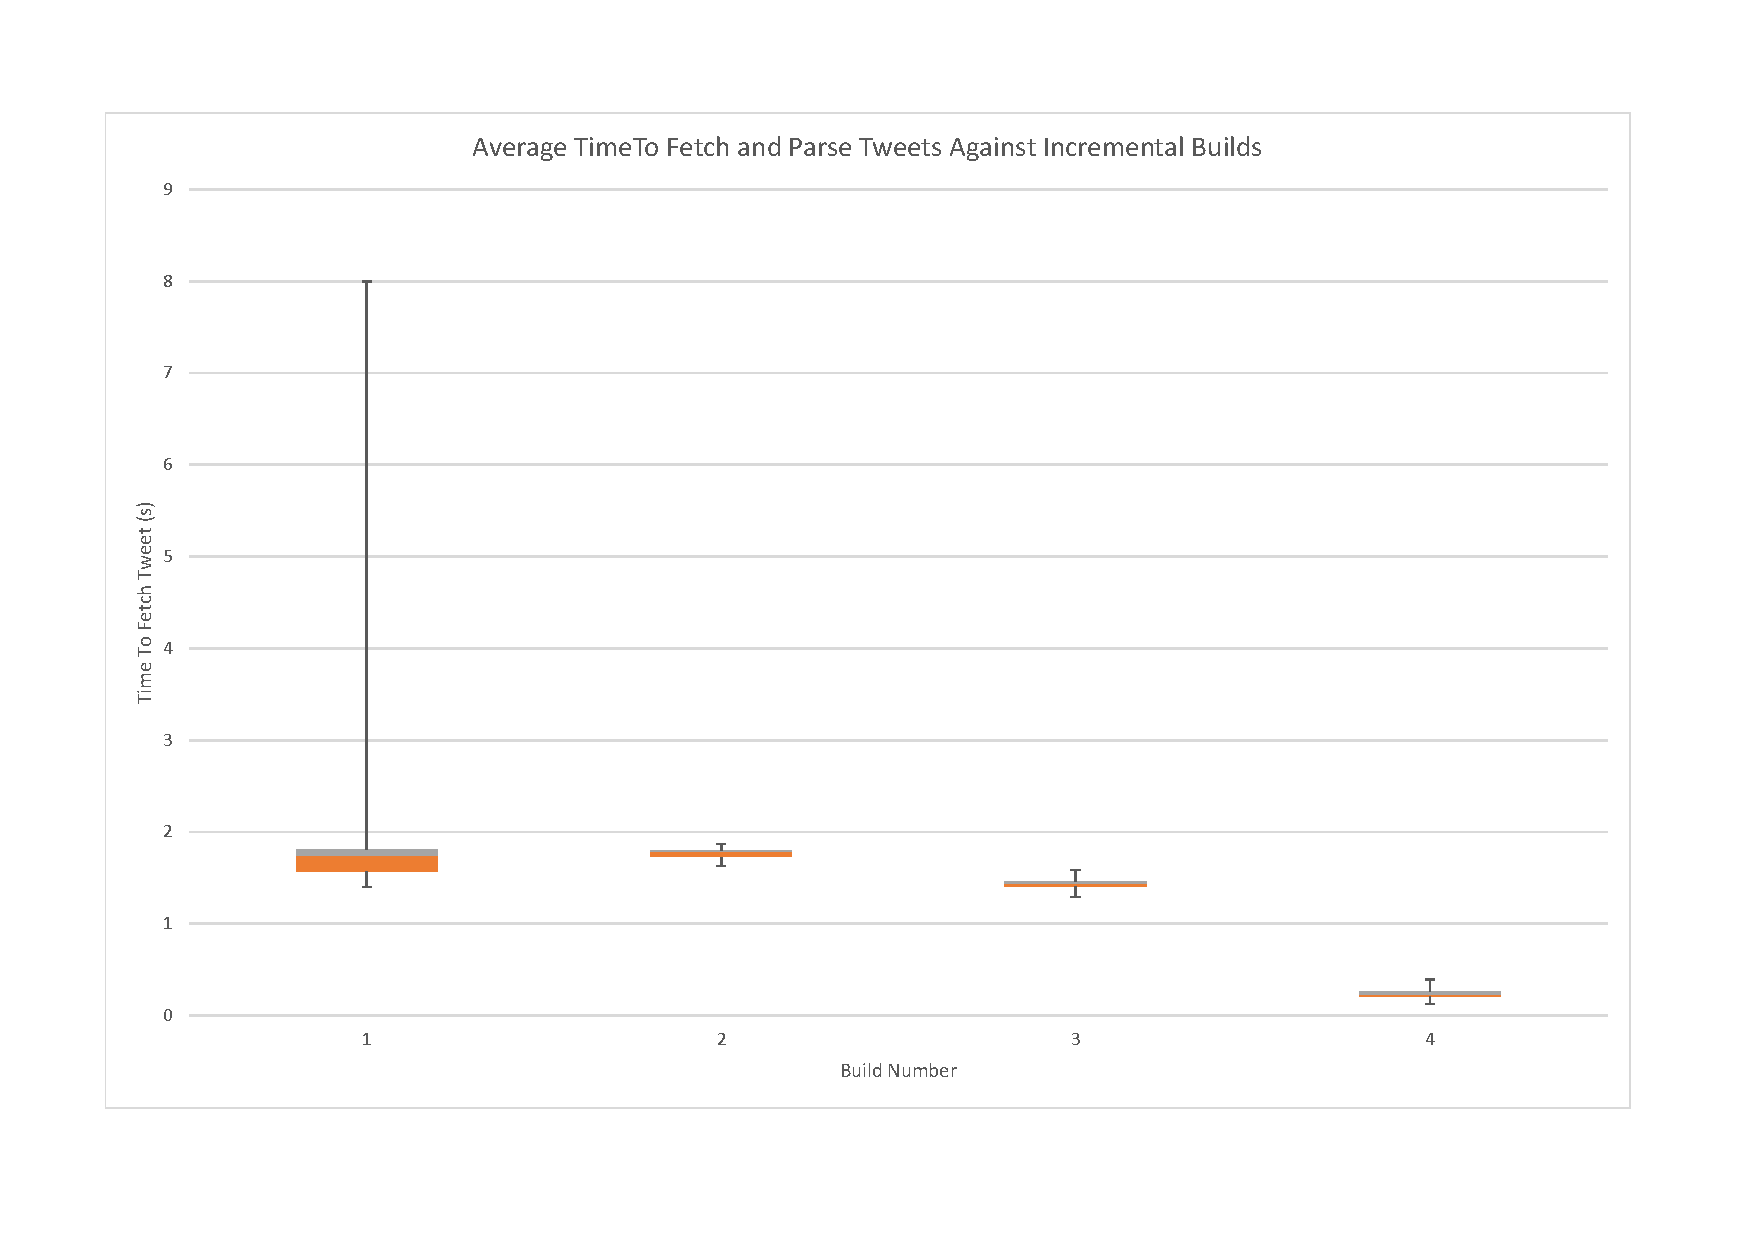
\includegraphics[width=500px]{Images/scrape_performance_against_builds.pdf}
\caption{Scraper performance improvements across incremental builds.}
\end{figure}
\end{center}
%Performance testing for the Twitter scraper is conducted using quantitative performance data, collected at the end of each build. The primary metric for scraper efficiency is average time to scrape and parse a tweet. 

%Figure 7.2 demonstrates the performance gains that 

% Performance benefits were experienced at the end of each development iteration, which was positive. 

% Talk about causes for large increases in performance, as well as the reason for a large outlier on the first builds

% Talk about how parallel implementation resulted in a order of magnitudinal increase in performance. 

\subsection{Resulting Policy Performance}

Based upon the final build results, I am able to evaluate performance of the examplar policies proposed in chapter 6. As policies must fetch the entire profile to generate the impact factor calculation, time to fetch profiles is the primary metric against which I evaluate policy performance. The analysis components calculating impact factor perform on the order of one to two seconds, depending on profile size. Thus I measure policy performance entirely against profile fetch times, as these are by far the most time-consuming factor to reputation metric calculation. The average time to fetch profiles is shown in figure \textbf{x}, using the parallel performing build. Despite the time taken to fetch a single tweet having been dramatically reduced in this version, an entire profile still takes hundreds of seconds on average.

Therefore I conclude requirement NF2 to not have been met, as policies resulting from are too slow for use in a real-time system. In the Twitter case study this is due to the necessity for a seperate HTTP request to fetch every single tweet. Although parrelisation of tweet fetching greatly improved performance, this requirement was largely infeasible. for websites with more static content such as LinkedIn, I propose that this would be possible however. 

\begin{center}
\begin{figure}[h!]
\centering
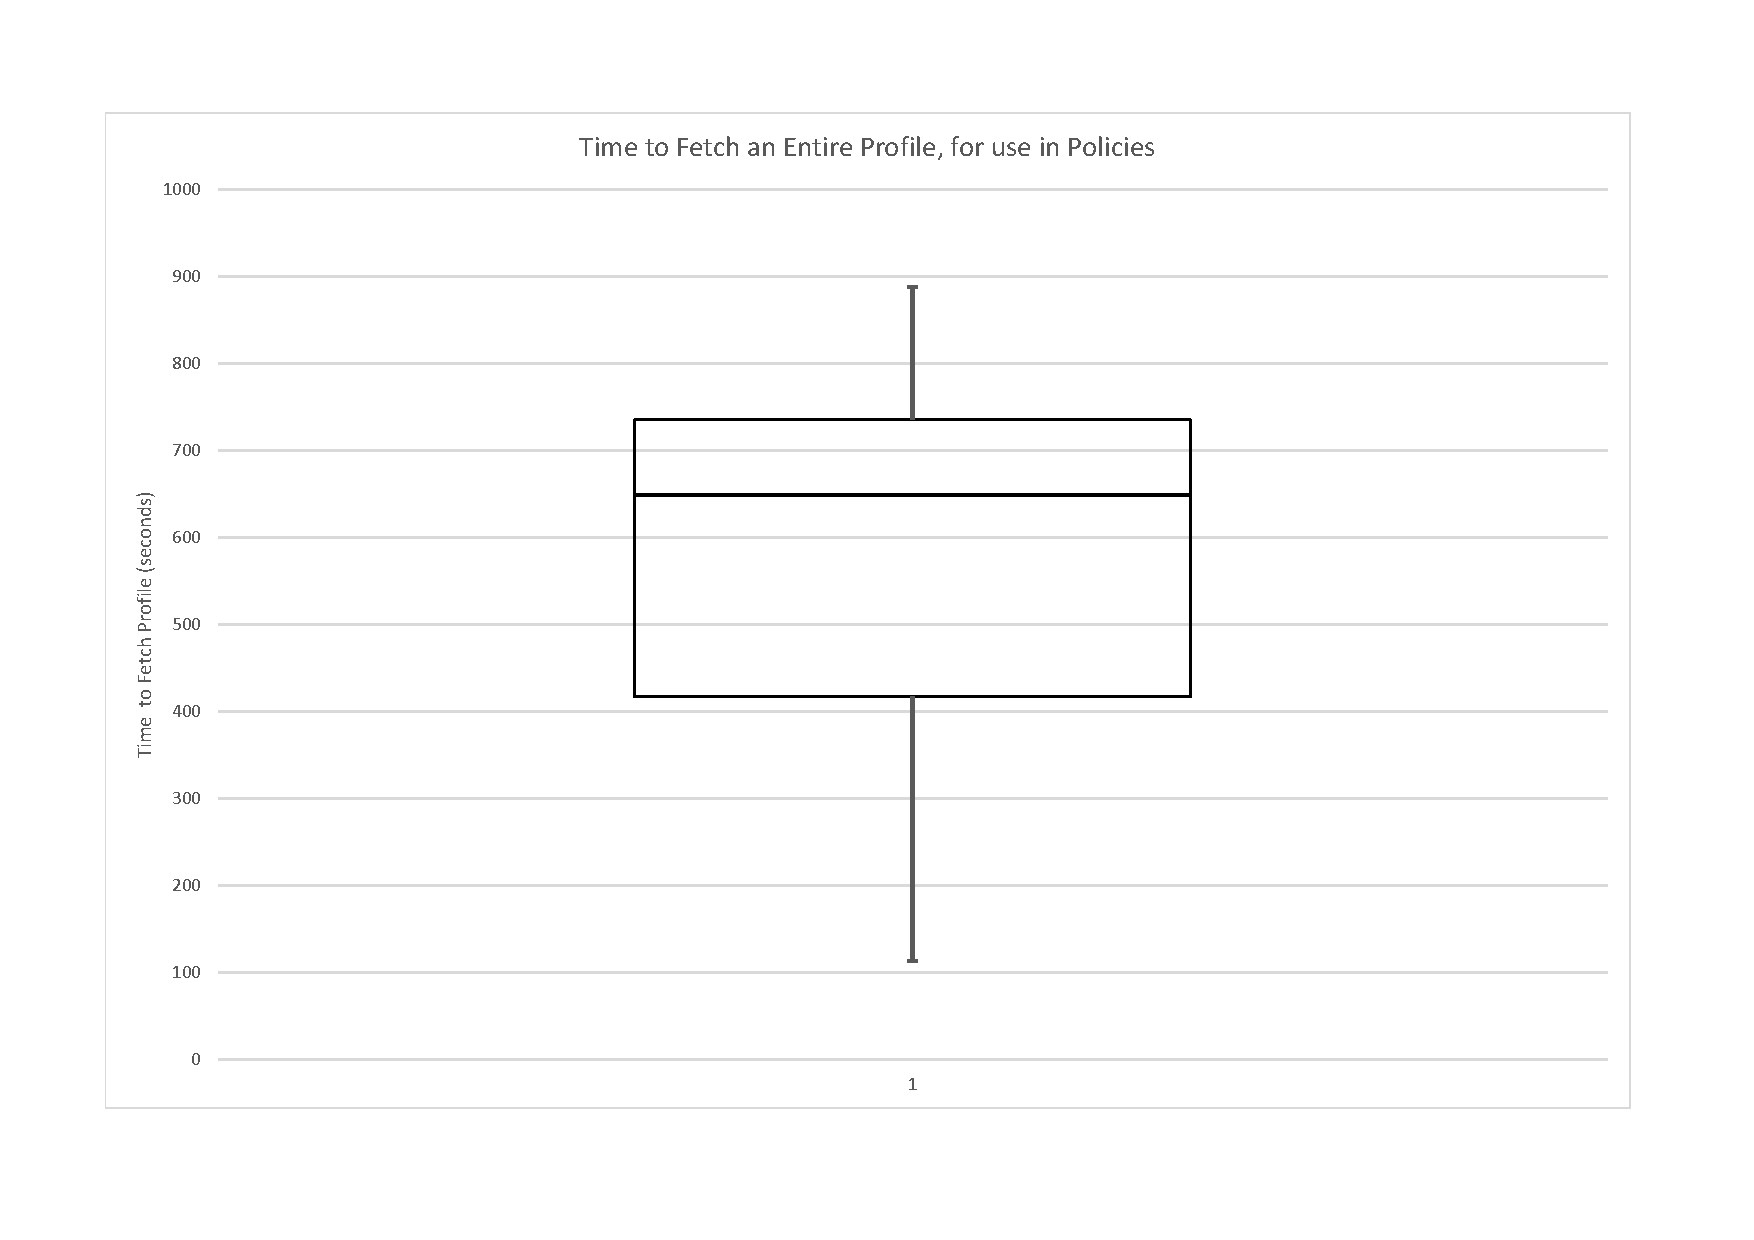
\includegraphics[width=500px]{Images/Average_Time_To_Fetch_Profile.pdf}
\caption{Average Times to Fetch an Entire Twitter Profile, for use in Policies}
\end{figure}
\end{center}



%Although this fetching was parrelised, increasing performance sixfold

%The average time to fetch profiles is shown in figure .

%The analysis components calculating impact factor perform much faster, on the order of one to two seconds, depending on 

%Based upon the final build results, we are able to evaluate the performance and practicality of policy fragments defined in chapter 6. 

%For each policy, discuss how long this would take on average for an average profile.

%Average number of tweets, and average time to fetch and parse a tweet based upon build number. 

\section{Resistance to Interface Change}

Evaluation of scraper resistance to interface change was conducted qualitatively. I summarise the critical points which, if changed, would result in the scraper failing. Discussion of the likelihood of these components changing is conducted in order to asess their reliability. 

IHPScrape is reliant on two components remaining constant; URLs to fetch resources and xPath expressions to fetch specific values. URLs are less likely to change, as this implies some level of large backend change or migration. xPath expressions are much more brittle, especialy when hard-coded based upon document structure (for example document/v1/li/test/ is more brittle than //**[li]). To evaluate the resistance of my Twitter scraper against user interface or backend change, I constructed a summary of all hard-coded URL and xPath expressions used to fetch data.

\begin{figure}[h!]
\begin{center}
  \begin{tabular}{| p{9cm} | l | }
  \hline
   \textbf{Feature} & \textbf{Nature of Dependancy}  \\ \hline
   Google Twitter Search - searching for Twitter profiles by name. URL is modified to input name parameter. & URL \\ \hline
   Twitter base profile. URL is modified to search for Twitter page with given user name. & URL \\ \hline
   Fetch extra tweets. Backend HTTP request to load more tweets for the current profile. & URL  \\ \hline
   Fetch tweet detail. HTTP request to load tweet detail for the current tweet, using ID as a parameter.& URL \\ \hline
   Fetch retweeter list. HTTP request to fetch the retweeters for the current tweet, using ID as a parameter.& URL \\ \hline
   Google Twitter Search - retrieve names. The names are located at specific points on the result page.& xPath \\ \hline
   Fetch core profile statistics. Name, number of tweets, number of followers, number following.&  xPath \\ \hline
   Fetch detailed tweet information. Retweets, favourites, favourites, content, date\_time.&  xPath \\ \hline
   Fetch retweeter names. &xPath \\ \hline
  \end{tabular}  
\end{center}
\caption{Scraper Interface Dependancies}
\end{figure}
%Best represented in a table?

Taken in the context of the entire scraper, the number of absolute interface dependancies is low. Over the course of the project, the Twitter user interface did not change, nor the URL structure. As such it is difficult to test whether any change would genuinely result in the scraper breaking, and how difficult this change would be to fix. From the analysis performed, I conclude that requirement NF1 was met; small changes should not result in the scraper breaking, unless they affect the specific points of failure outlined in figure 7.3. Wholesale interface redesigns will of course result in scrapers breaking, but such resistance was deemed infeasible. %Finish this.
%Fix this up. Tomorrow.
%Discuss how likely each of these components is to change
%State that any change would result in the scraper breaking
%Google twitter search - URL reliance
%To evaluate scraper and framework resistance 
%Metric evaluation based upon fields that may change, and the effects that would occur if these changes happened.
%Heuristic discussion of the fields which would result in scrapers breaking. 

\section{Resistance to Detection}

Evaluation of scraping detection was performed throughout the data collection phase, by logging events where a scraper was blocked. The primary event indicating Twitter had blocked or limited my scraper was primarily the 503 error code. This has been experienced by other Twitter scrapers, confirming that this code indicates rate limiting and not a coding failure. The secondary event recorded to indicate blocking was 500 error codes - this was in fact a mistake, as 500 errors were in response to coding errors in IHPScrape.

Figure 7.4 shows the percentage of failed profiles against incremental builds for the Twitter scraper. The definition of failure here is a profile that was not fetched in its entirety. As such the rates of failure look worse than is the case. In the first build, the parsing code was not sufficiently reliable, and in many cases parse errors were encountered midway through scraping a profile. These were for special case events such as photo posts that I had not considered. The second build vastly improved the parsing quality, and gave way to detection issues, which were in turn subsequently reduced. The final build had an extremly small percentage of genuinely failed profiles, and only approximately 1 in 10 profiles not entirely fetched. As mentioned earlier, many incomplete profiles are of such size that further fetching is somewhat redundant. 

I conclude that the requirement F4 was half met. The final Twitter build demonstrates that mechanisms in place to avoid detection were effective, as only extremly large profiles result in detection and incompleteness. However recovery from failure was not implemented for Twitter, as it was impossible to distinguish for example the end of a profile and the Twitter server responding with false information. 

%Scraping detection and failure rates were recorded at the end of each build phase, displaying the incremental gains resulting from my development approach. The first build had extremely high parse errors, caused by choice of parsing library - this was one of the issues with feasibility noted at the milestone report. Having improved parsing... %Blah blah

\begin{center}
\begin{figure}[h!]
\centering
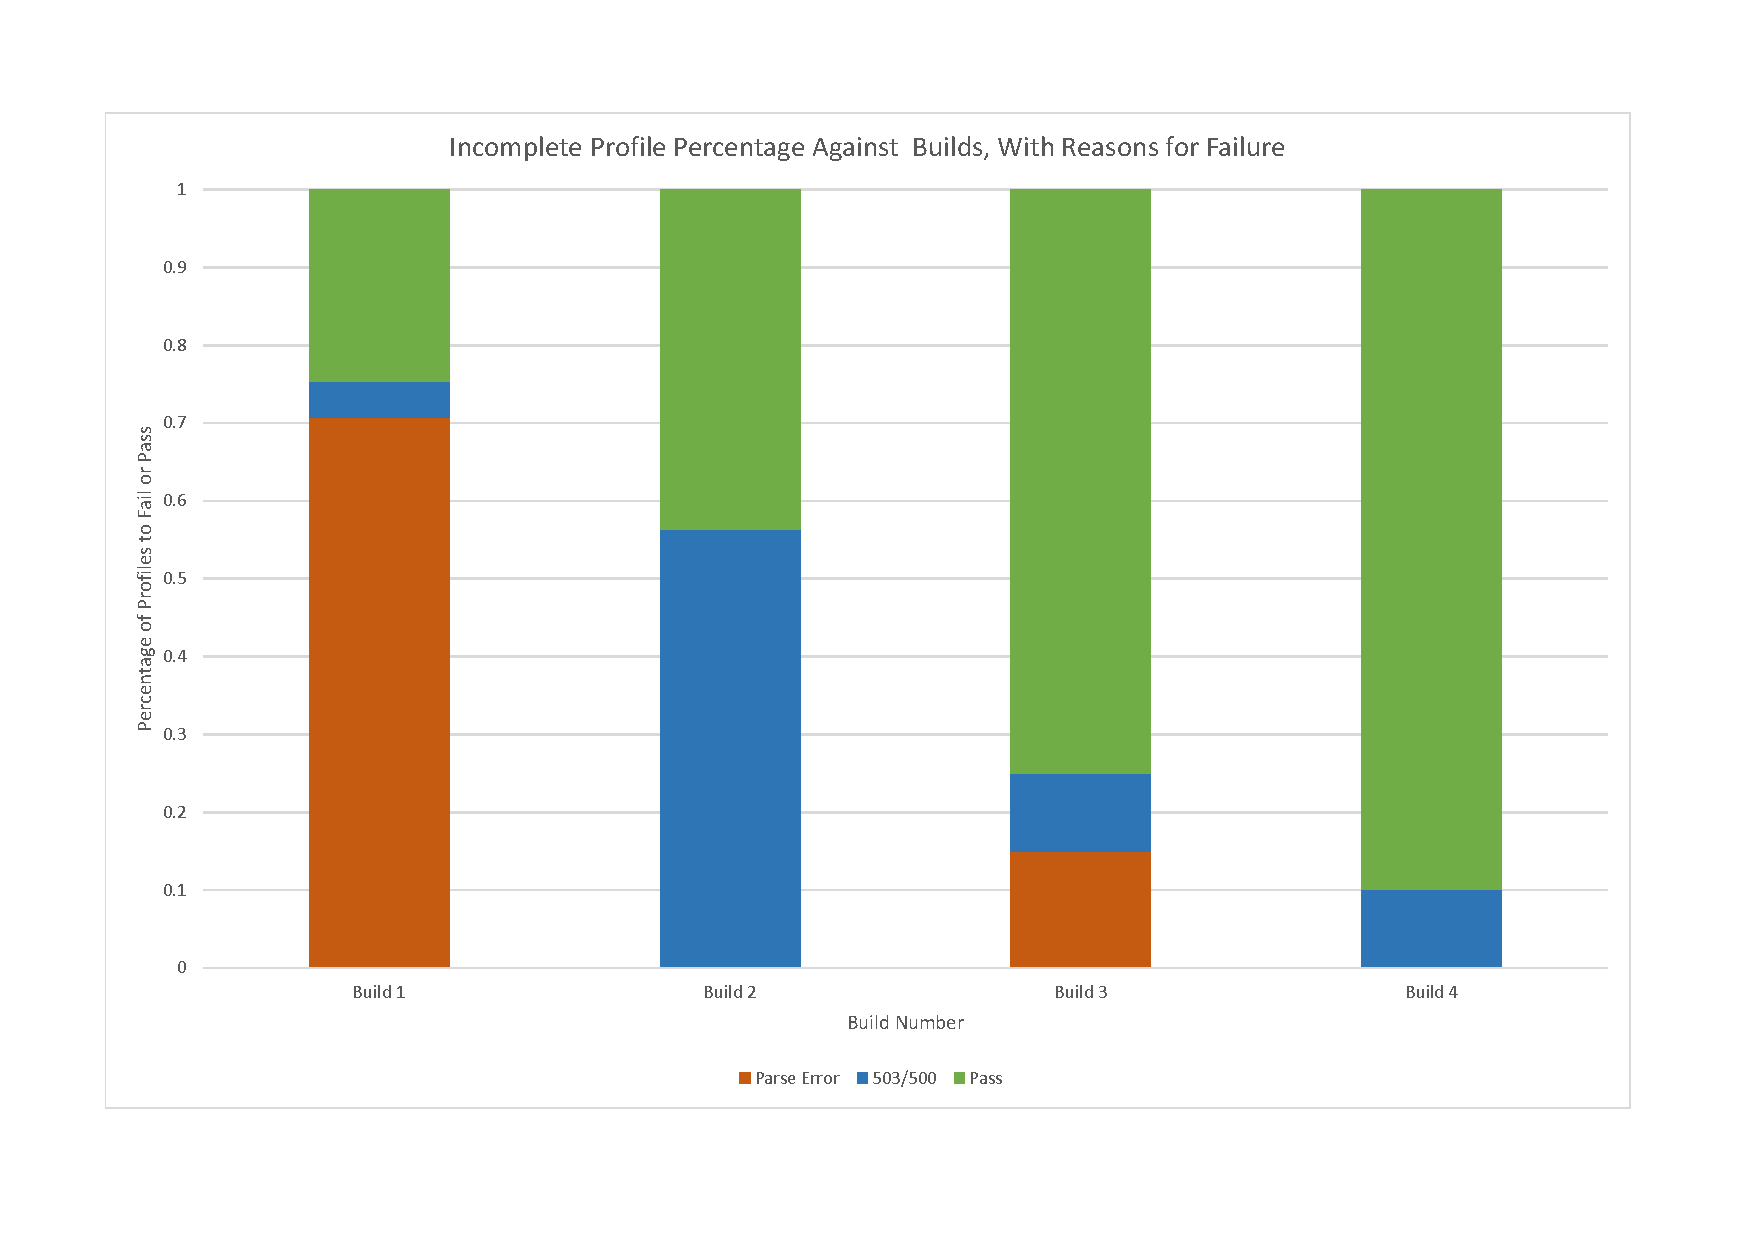
\includegraphics[width=500px]{Images/failure_rate_and_reason.pdf}
\caption{Incomplete profiles fetched, with reasons for Failure.}
\end{figure}
\end{center}

%\section{Extensibility and Social Media Portability of Scraping Framework - LinkedIn Case Study}

%The development of a LinkedIn scraper is a suitable case study to evaluate the social media portability of the IHPScrape framework. Development of this scraper was completed in one weeks work, compared to the 

%How the framework helps in development of social media scarpersTje

%What improvements could have been made to the scraper.s

%I qualitatively evaluate the social media portability of the scraping framework, with respect to the case study of developing a LinkedIn scraper. 

%Discuss with associated heuristics the development of the LinkedIn scraper, and how the framework assisted with the development of this scraper. %#BULLSHIT BULLSHIT BULLSHIT!

%Performance testing of scrapers was carried out throughout the project, through performance logging mechanisms designed to measure the time taken to fetch an entire profile. To reduce bias caused by varying network speeds at University, the software was run over extended periods of time.
%Given the iterative approach taken to develop the scrapers, I evaluate their performance with respect to incremental builds, as well as final performance. As the definition of a 'profile' differs between sites, different performance metrics are used for each site. 
